\documentclass[10pt,a4paper]{article}
\usepackage[T1]{fontenc}
\usepackage[utf8]{inputenc}
\usepackage{lmodern}
\usepackage[margin=0.82in]{geometry}
\usepackage{amsmath,amssymb,bm,booktabs,array,tabularx}
\usepackage{graphicx,caption,xcolor,hyperref,tikz}
\usetikzlibrary{arrows.meta,positioning}
\hypersetup{colorlinks=true,linkcolor=blue!45!black,citecolor=blue!45!black,urlcolor=blue!45!black,
pdftitle={Robust QCar State Estimation with Analytical Consistency Gates and Learned Measurement Trust}}
\graphicspath{{paper_assets/}}
\captionsetup{font=small,labelfont=bf}
\setlength{\parskip}{3pt}
\setlength{\emergencystretch}{2em}
\renewcommand{\arraystretch}{1.13}
\newcommand{\vx}{\bm{x}}
\newcommand{\vz}{\bm{z}}
\newcommand{\wrap}{\operatorname{wrap}}
\newcommand{\clip}{\operatorname{clip}}
\newcommand{\relu}{\operatorname{ReLU}}
\newcommand{\sigmoid}{\operatorname{sigmoid}}
\title{\vspace{-1.1em}Robust QCar State Estimation with Analytical\\
Consistency Gates and Learned Measurement Trust}
\author{Quang Huy Nugyen \and Echrak Chnib}
\date{}
\begin{document}
\maketitle
\vspace{-1.4em}
\begin{abstract}
Sensor corruption can degrade vehicle localization even when the nominal motion model is accurate.
This paper presents a hybrid QCar estimator combining a calibrated physical predictor,
explicit consistency checks, and a learned measurement-reliability model.
A shared neural network with 337 parameters modulates diagonal analytical correction gains;
it does not estimate an unrestricted Kalman gain matrix.
Sensor availability, inferred reliability, and the simulator's attack indicator are defined separately.
Only corrupted sensor measurements, commands, and their causal history enter online inference.
Training uses simulated drives with known corruption and state targets, while evaluation uses
continuous trajectories with disjoint drive seeds and no intermediate truth resets.
Across 13 nominal clean/fault conditions, the estimator has lower position RMSE than
the repository EKF. For GPS jumps, pooled position RMSE decreases from 0.7308 to 0.0139 m;
for gradual GPS drift it decreases from 0.5975 to 0.0701 m.
A neural ablation obtains 0.0142 and 0.2202 m, respectively, showing that analytical
design explains most jump rejection, whereas learning contributes more to gradual drift.
Separate Stanley--PID control experiments assess the effect on driving.
A combined GPS/tachometer attack under calibration mismatch increases hybrid error to
0.4638 m, above the analytical ablation's 0.4019 m.
The results establish an empirical improvement in the tested simulator, with explicit
limits on model mismatch, learning attribution, and transfer to physical vehicles.
\end{abstract}
\noindent\textbf{Keywords:} vehicle state estimation; sensor faults; measurement reliability;
hybrid filtering; QCar simulation; causal evaluation.

\section{Introduction}
A vehicle estimator must reject unreliable sensor information without losing the motion
information required by its controller. This is more demanding than smoothing nominal
measurement noise. A biased or frozen sensor can remain syntactically valid, and its
repeated corrections can move the estimate until the corrupted value becomes consistent
with the estimate itself. A corrupted tachometer or inertial signal can also affect
prediction before a position update is considered.

KalmanNet combines a structural state-space model with recurrent neural gain computation
for partially known dynamics \cite{revach2022}.
RobustStateNet models sensor branches with recurrent networks and selective feature fusion
within a prediction/update architecture \cite{dahal2024}.
These works motivate combining physical structure and learned reliability, but they do not
imply that a particular local implementation is robust to the QCar fault distribution.
The method studied here retains the repository name \texttt{RobustKLNet}, with the
backend identifier \texttt{innovation\_trust}. Its active architecture is a physical
predictor with analytical diagonal gains and learned trust, rather than the earlier
GRU gain network.

The contribution is an implemented and evaluated design for this simulation setting:
(i) consistency checks protect both prediction and correction;
(ii) analytical rejection and learned reliability are combined explicitly;
and (iii) continuous estimation and feedback-control experiments separate overall
performance from the incremental contribution of learning.
The study is an empirical engineering evaluation. It does not claim a new general
optimal filter, a formal attack-identification guarantee, or superiority to all robust
Kalman-filter variants.

\section{Estimation problem and information available online}
The state and direct measurement vector are
\begin{equation}
 \vx_k=[x_k,y_k,\psi_k,v_k]^\top,\qquad
 \vz_k=[x_k^{\rm GPS},y_k^{\rm GPS},\psi_k^{\rm GPS},v_k^{\rm tach}]^\top .
 \label{eq:state}
\end{equation}
The online inputs additionally include throttle $u_k$, the steering signal $\delta_k$,
yaw rate $\omega_k^{\rm IMU}$, longitudinal acceleration $a_k^{\rm IMU}$, and the
sample interval $\Delta t_k$. Angular differences are wrapped to $[-\pi,\pi)$.
GPS heading is checked before it can contaminate a separate heading-fusion stage.
The tachometer is one physical source; four repeated copies are not treated as
independent wheel observations.

For an available channel, a useful fault notation is
\begin{equation}
 z_{k,j}=h_j(\vx_k)+n_{k,j}+d_{k,j},
 \label{eq:corruption}
\end{equation}
where $d_{k,j}$ denotes corruption. Replacement and freeze faults can be represented
by a time-dependent $d_{k,j}$; dropout instead removes the observation.
The estimator does not observe $d_{k,j}$, the clean counterpart, the true moving state,
or the scheduled attack interval. Its initialization uses the known spawn pose once.

\begin{table}[htbp]
\centering\small
\caption{Three distinct quantities: attack annotation, availability, and inferred trust.}
\label{tab:mask}
\begin{tabularx}{\linewidth}{@{}l l X@{}}
\toprule
Quantity & Values & Meaning and use\\
\midrule
Attack indicator $A_k$ & $\{0,1\}$ & Known only to the experiment generator and scorer;
$1$ marks an injected fault interval. It is not an inference input.\\
Availability $a_{k,j}$ & $\{0,1\}$ & Obtained from sensor validity/freshness metadata and
finite-value checks. A corrupted observation may still have $a_{k,j}=1$.\\
Applied trust $\gamma_{k,j}$ & $[0,1]$ & Computed online. A small value suppresses
that measurement's correction; it is not the attack signal or a calibrated
probability of malicious activity.\\
\bottomrule
\end{tabularx}
\end{table}

\section{Hybrid estimator}
\subsection{Calibrated prediction and protection of motion inputs}
Let $F(v,u,\Delta t)$ be the calibrated throttle-to-speed propagation.
For the evaluated lookup model,
\begin{align}
 v_{\rm ss}(u)&=\operatorname{interp}(u;\mathcal U,\mathcal V),&
 \dot v_0&=\frac{v_{\rm ss}(u)-v}{\tau}, \nonumber\\
 \dot v&=\clip\!\left(\dot v_0,-2,\frac{2v_{\rm sw}}{\max(v,v_{\rm sw})}\right),&
 F(v,u,\Delta t)&=\clip(v+\Delta t\,\dot v,-2.5,2.5).
 \label{eq:speed}
\end{align}
The nominal constants are $\tau=0.301$ s, $v_{\rm sw}=0.1$ m/s and wheelbase $L=0.26$ m.
Acceleration limits are in $\mathrm{m/s^2}$.
A near-stop rule sets acceleration to zero when $|u|<0.01$ and $|v|<0.03$ m/s.
Appendix~\ref{app:parameters} gives the static lookup points supplied as nominal
calibration to both plant and estimators.

Two velocities are propagated:
$v_k^-=F(\hat v_{k-1},u_k,\Delta t_k)$ and a command-driven auxiliary velocity
$v_k^{\rm cmd}=F(v_{k-1}^{\rm cmd},u_k,\Delta t_k)$.
The latter receives no direct tachometer correction.
The tachometer's influence on pose prediction is moderated by
\begin{align}
 q_k&=\exp\!\left[-\min\left\{
       \left(\frac{|v_k^{\rm tach}-v_k^{\rm cmd}|}{0.20}\right)^4,60\right\}\right]
       \gamma_{k-1,v}, \nonumber\\
 v_k^{\rm use}&=v_k^-+0.65q_k(v_k^{\rm tach}-v_k^-).
 \label{eq:tach}
\end{align}
The previous-trust factor is omitted at the first sample.
A non-finite or detected frozen tachometer sets $q_k=0$.
Rejection therefore protects motion prediction as well as the velocity update.

A first-order, rate-limited steering state follows the steering input.
Its bicycle yaw-rate prediction is compared with the IMU yaw rate and acceleration.
The predictor uses the IMU rate when consistency tests accept it and otherwise uses
the bicycle rate. Appendix~\ref{app:guards} specifies these deterministic guards.
With accepted yaw rate $\omega_k$ and midpoint speed
$\bar v_k=(\hat v_{k-1}+v_k^{\rm use})/2$, the prediction is
\begin{equation}
 \vx_k^-=
 \begin{bmatrix}
 \hat x_{k-1}+\bar v_k\Delta t_k\cos(\hat\psi_{k-1}+\omega_k\Delta t_k/2)\\
 \hat y_{k-1}+\bar v_k\Delta t_k\sin(\hat\psi_{k-1}+\omega_k\Delta t_k/2)\\
 \wrap(\hat\psi_{k-1}+\omega_k\Delta t_k)\\
 v_k^-
 \end{bmatrix}.
 \label{eq:prediction}
\end{equation}
These equations describe the evaluated kinematic regime, not a learned tire/slip model.

\subsection{Odometry reference and temporal features}
An auxiliary state $\bm{o}_k$ is integrated using accepted speed and yaw rate,
without the fast GPS position corrections. Its velocity is $v_k^{\rm cmd}$.
Persistent GPS displacement can thus remain visible even after the main estimate begins
moving toward that displacement. This reference is \emph{not statistically independent}:
it shares motion inputs and accepted speed history with the main estimate.

The innovation and reference discrepancy are
\begin{equation}
 r_{k,j}=z_{k,j}-x_{k,j}^-,\qquad d^o_{k,j}=z_{k,j}-o_{k,j},
 \label{eq:residuals}
\end{equation}
with angular wrapping in channel $\psi$.
Successive available observations and their corresponding reference states give
a motion-disagreement feature $\Delta z_j-\Delta o_j$.
An exponentially weighted discrepancy is updated on available samples as
$E_{k,j}=0.85E_{k-1,j}+0.15d^o_{k,j}$.
Unavailable channels retain their history.

Each channel has a 12-dimensional feature vector
\begin{equation}
 \bm f_{k,j}=
 \begin{bmatrix}
 \log(1+|r_{k,j}|/s_j)\\
 \log(1+|d^o_{k,j}|/s_j)\\
 \log(1+|\Delta z_j-\Delta o_j|/s_j)\\
 \log(1+|E_{k,j}|/s_j)\\
 \min(T^{\rm repeat}_{k,j},3)\\
 |v_k^{\rm use}|\\
 |\omega_k|\\
 \min(\Delta t_k^{\rm GPS},2)\\
 \bm e_j
 \end{bmatrix},
 \qquad \bm s=[0.12,0.12,0.09,0.10]^\top ,
 \label{eq:features}
\end{equation}
where $\bm e_j$ is a four-entry channel identity vector.
$T^{\rm repeat}$ is an implementation-level repeated-value accumulator; its timing
convention and the separate tachometer timer are stated in Appendix~\ref{app:guards}.
The features contain current measurements and past information only.

\subsection{Analytical consistency and learned measurement trust}
A shared MLP evaluates all four channels:
\begin{equation}
 \rho_{k,j}=\sigmoid\!\left(W_2\relu(W_1\bm f_{k,j}+\bm b_1)+b_2\right).
 \label{eq:mlp}
\end{equation}
Here $W_1\in\mathbb R^{24\times12}$ and $W_2\in\mathbb R^{1\times24}$,
giving $288+24+24+1=337$ trainable parameters.
Memory resides in the filter and its features; the MLP itself is not recurrent.

The deterministic consistency term is
\begin{align}
 e_{k,j}&=\max\{|r_{k,j}|,0.75|d^o_{k,j}|\},\nonumber\\
 b_{k,j}&=\exp\!\left[-\min\left\{(e_{k,j}/c_j)^4,60\right\}\right],
 & \bm c&=[0.30,0.30,0.20,0.20]^\top .
 \label{eq:prior}
\end{align}
The entries of $\bm c$ are in metres, metres, radians and metres per second.
Explicit frozen-sensor guards can set affected $b_{k,j}$ to zero.
This rule strongly suppresses large discrepancies rather than repeatedly applying
a fixed clipped residual. Availability, consistency and learning are combined:
\begin{align}
 \tilde\gamma_{k,j}&=a_{k,j}b_{k,j}\rho_{k,j},&
 \gamma_{k,x}=\gamma_{k,y}&=\min(\tilde\gamma_{k,x},\tilde\gamma_{k,y}),\nonumber\\
 \gamma_{k,\psi}&=\tilde\gamma_{k,\psi},&
 \gamma_{k,v}&=\tilde\gamma_{k,v}.
 \label{eq:trust}
\end{align}
GPS position is treated as a pair. This avoids retaining one coordinate when the
other indicates an unreliable position source. It does not assert statistical
independence of heading, velocity and position errors.

\begin{figure}[htbp]
\centering
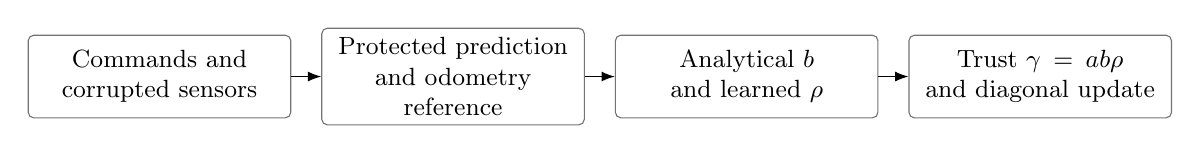
\begin{tikzpicture}[>=Latex,
 box/.style={draw=black!55,rounded corners=2pt,align=center,text width=3.1cm,
 minimum height=1.05cm,font=\small},node distance=0.38cm]
\node[box] (a) {Commands and\\corrupted sensors};
\node[box,right=of a] (b) {Protected prediction\\and odometry\\reference};
\node[box,right=of b] (c) {Analytical $b$\\and learned $\rho$};
\node[box,right=of c] (d) {Trust $\gamma=a b\rho$\\and diagonal update};
\draw[->] (a)--(b);\draw[->] (b)--(c);\draw[->] (c)--(d);
\end{tikzpicture}
\caption{Online computation. Temporal states feed the next prediction and trust features.
Attack indicators and clean references are absent from this inference path.
The shared GPS-position minimum in Eq.~\eqref{eq:trust} precedes correction.}
\label{fig:architecture}
\end{figure}

\subsection{Analytical correction and its limited guarantee}
Four positive variance-like scalars determine the gains:
\begin{align}
 P_{k,j}^-&=P_{k-1,j}^++Q_j\frac{\Delta t_k}{0.02},&
 K_{k,j}&=\frac{P_{k,j}^-}{P_{k,j}^-+R_j},\nonumber\\
 \alpha_{k,j}&=K_{k,j}\gamma_{k,j},&
 \hat x_{k,j}&=x_{k,j}^-+\alpha_{k,j}r_{k,j},\label{eq:update}\\
 P_{k,j}^+&=\max\{(1-\alpha_{k,j})P_{k,j}^-,10^{-9}\}.&&\nonumber
\end{align}
Heading is wrapped after correction. Appendix~\ref{app:parameters} specifies the
initial variances, $Q_j$ and $R_j$.
The recursion omits Jacobian-based cross-covariance propagation and uses $P$ as a
gain-scheduling quantity; it is not established as a calibrated posterior covariance
or an optimal EKF recursion.

Since $P^->0$, $R>0$ and $\gamma\in[0,1]$, one has $0\leq\alpha<1$.
For a non-angular channel the direct correction is a convex interpolation between
prediction and measurement; for heading the same property holds along the wrapped residual.
The diagonal update prevents a position residual from \emph{directly} correcting
heading or velocity in that update.
This local algebraic property does not prove bounded trajectory error, attack detection,
or global stability. Subsequent prediction still couples the states.

After correction, each reference pose coordinate is slowly aligned only if
$\gamma_{k,j}>0.8$ and $|d^o_{k,j}|<0.65s_j$:
\begin{equation}
 o_{k,j}\leftarrow o_{k,j}
 +\min(\Delta t_k^{\rm GPS}/8,0.1)d^o_{k,j},\qquad j\in\{x,y,\psi\}.
 \label{eq:align}
\end{equation}
This reduces nominal drift while limiting rapid assimilation of suspicious GPS offsets.
Coherent slow corruption can nevertheless contaminate the shared reference.

\subsection{Relationship to the previous implementation}
The retained legacy implementation has a learned feature/measurement mask and a recurrent
gain calculation. The active backend replaces that recurrent gain with Eq.~\eqref{eq:update},
uses the physical predictor of Eq.~\eqref{eq:prediction}, and learns only $\rho$.
It also checks GPS heading before fusion, rejects frozen tachometer influence in prediction,
and disables publication of a clean-reference comparator as the estimator output.
The persistent concept is prediction followed by reliability-weighted correction.
The architectural change separates explicit safeguards, analytical gains and a smaller
learned component.

\section{Learning measurement reliability}
\subsection{Offline supervision}
A training drive contains clean noisy sensor samples, corrupted samples and simulated true
states. These are available to the training-data generator only.
Let $\epsilon_{k,j}^{\rm fault}=z_{k,j}^{\rm corrupt}-z_{k,j}^{\rm clean}$
with heading differences wrapped. Soft reliability targets are
\begin{equation}
 y_{k,j}=\exp[-(|\epsilon_{k,j}^{\rm fault}|/\eta_j)^2],
 \qquad \bm\eta=[0.07,0.07,0.05,0.06]^\top .
 \label{eq:target}
\end{equation}
The two position targets are replaced by their minimum.
A frozen value can retain high target reliability until it departs materially
from the contemporaneous clean measurement.
Unavailable measurements are excluded from the training examples.
The generator's binary attack labels are not the network inputs or the direct targets
of this objective.

Training uses six drive seeds (1--6), and model selection uses two disjoint seeds (21--22).
Drives last 30 s at 50 Hz. GPS rates cycle through 5, 10 and 20 Hz.
The plant time constant varies by $-8\%,0,+8\%$ and the steady-state speed curve by
$-4\%,0,+4\%$, according to the seed, while estimator calibration remains nominal.
Each drive is replayed under the 13 conditions in Table~\ref{tab:faults}, including clean data.

\subsection{Corruption-weighted reliability and correction loss}
The reliability term is weighted binary cross entropy:
\begin{equation}
 \mathcal L_{\rm rel}
 =-\frac{1}{M}\sum_i [1+3(1-y_i)]
       \big[y_i\log\rho_i+(1-y_i)\log(1-\rho_i)\big].
 \label{eq:bce}
\end{equation}
This is corruption weighting, not exact balancing by class frequency.
The index $i$ spans available channel observations.

A second term measures a candidate one-step correction on stored rollout features.
For normalization scales $\bm\ell=[0.04,0.04,0.02,0.025]^\top$, define
$\bar r_i=r_i/\ell_j$ and
$\bar e_i=(x_i^- -x_i^{\rm true})/\ell_j$, with angular wrapping.
The data-collection filter stores
\begin{equation}
 \bar g_i=\frac{K_i\gamma_i^{\rm collect}}
                  {\max(\rho_i^{\rm collect},10^{-6})},
 \qquad
 \mathcal L_{\rm state}=\frac{1}{M}\sum_i
          \min\{(\bar e_i+\rho_i\bar g_i\bar r_i)^2,100\}.
 \label{eq:state_loss}
\end{equation}
The total loss is
\begin{equation}
 \mathcal L=\mathcal L_{\rm rel}+0.08\mathcal L_{\rm state}.
 \label{eq:loss}
\end{equation}
Collected gains, the reference state and GPS-position coupling are fixed while optimizing
each minibatch. Equation~\eqref{eq:state_loss} is thus a local surrogate, not differentiation
through the full filter trajectory or through the current two-coordinate minimum.
The clipping limits the influence of large state errors on this loss.

\subsection{Two collection/training passes}
The first pass collects features using the analytical filter with $\rho=1$.
After fitting the MLP, the second pass recollects causal features using the first learned
checkpoint and continues optimization. This exposes training to states visited by a
learned filter; it does not eliminate train/deployment distribution mismatch.

Optimization uses AdamW with learning rate $0.003$, weight decay $10^{-4}$, batch size
4096, gradient-norm clipping at 2, and training seed 17.
Each pass permits 60 epochs. An improvement threshold of $10^{-5}$ and patience of
15 epochs govern early stopping; the best validation weights in each pass are restored.
Both recorded passes ran 60 epochs.
The selected epochs in Table~\ref{tab:training} use one-based numbering.
A lower second-pass loss is descriptive because its collected examples differ from the
first pass; the external continuous benchmark determines estimation quality.

\begin{table}[htbp]
\centering\small
\caption{Recorded losses at the selected epoch of each collection/training pass.}
\label{tab:training}
\begin{tabular}{lrrr}
\toprule
Pass & Selected epoch & Training loss & Validation loss \\
\midrule
1 & 60 & 0.07792 & 0.05920 \\
2 & 58 & 0.04374 & 0.03752 \\
\bottomrule
\end{tabular}

\end{table}
\begin{figure}[htbp]
\centering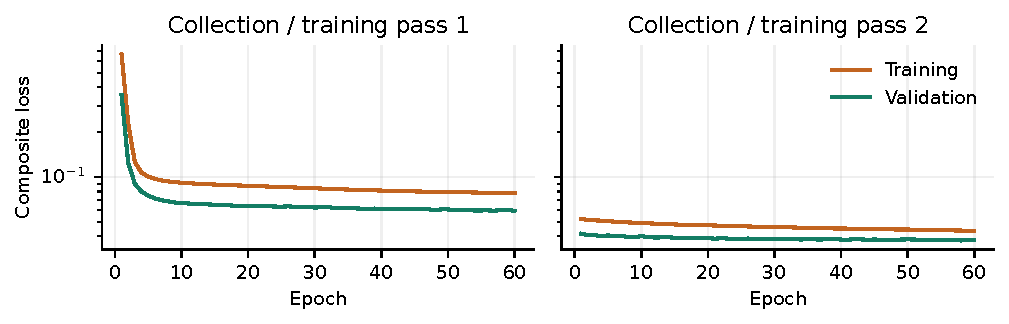
\includegraphics[width=.91\linewidth]{training_history.pdf}
\caption{Optimization histories from saved checkpoint metadata. The neural network is
trained on channel examples collected from causal rollouts; it is not an online
optimizer during evaluation.}
\label{fig:training}
\end{figure}

\section{Experimental protocol}
\subsection{Plant, sensors, and causal evaluation}
Experiments use the repository's \texttt{MockQCar} plant, also used by
\texttt{fake\_vehicle\_real\_logic.py}. The main benchmark uses its kinematic model,
calibrated throttle lookup and default steering actuator.
Throttle and steering commands vary sinusoidally with seed-dependent phases; a short
stop occupies approximately 72--78\% of each drive.
The electronics twin is disabled in these benchmarks.

The nominal test comprises seeds 101--103, 60 s per drive, $\Delta t=0.02$ s,
and 10 Hz GPS. Independent added sensor noise has standard deviations 0.035 m per
GPS coordinate, 0.015 rad for GPS heading, 0.012 m/s for tachometer speed,
0.008 rad/s for gyro rate, and 0.04 $\mathrm{m/s^2}$ per acceleration component.
Initial positions are zero, initial headings are seed-dependent, and speed starts at zero.
Each estimator receives the same corrupted samples and one known initial pose.
Its state remains continuous for all 3000 steps; no target reset or overlapping-window
averaging is performed.

The test seeds do not overlap training/validation seeds. However, the fault families and
command-generation family are represented during training.
These are tests on new drives within specified families, not demonstrations on
previously unseen attack mechanisms.
The saved seeds should not be reused as an untouched final test after further model tuning.

\subsection{Fault conditions}
For each non-clean open-loop condition, fault intervals are
$[0.22T,0.45T)$ and $[0.56T,0.70T)$: $[13.2,27.0)$ and $[33.6,42.0)$ s for $T=60$ s.
Each interval samples a sign $\varsigma\in\{-1,1\}$ and jump magnitude
$B\sim U(0.65,1.4)$ m. The schedule is external to the estimator.

\begin{table}[htbp]
\centering\small
\caption{Nominal open-loop conditions. Offsets are applied to estimator inputs after
plant simulation; steering corruption does not alter the plant command in this test.
$t_a$ is time since the current fault interval began.}
\label{tab:faults}
\begin{tabularx}{\linewidth}{@{}l X@{}}
\toprule
Condition & Injected change\\
\midrule
Clean & Nominal sensor noise only.\\
GPS jump & Position offsets $(\varsigma B,-0.7\varsigma B)$ m.\\
GPS ramp & Position offsets $(0.12\varsigma t_a,-0.08\varsigma t_a)$ m.\\
GPS freeze & Reuse the first GPS packet in the interval, including heading.\\
GPS dropout & Remove GPS packets, including GPS heading.\\
GPS noise & Add independent position noise with standard deviation 0.65 m.\\
Heading bias & Add $0.9\varsigma$ rad to GPS heading, then wrap.\\
Tachometer bias & Add $0.65\varsigma$ m/s to measured speed.\\
Tachometer scale & Multiply measured speed by 1.9.\\
Tachometer freeze & Hold the speed measurement at interval onset.\\
IMU bias & Add $0.8\varsigma$ rad/s to yaw rate and $1.5\varsigma$
$\mathrm{m/s^2}$ to each of the first two acceleration components.\\
Steering bias & Add $0.3\varsigma$ rad to the estimator's steering input.\\
GPS + tachometer & Combine GPS jump and tachometer bias.\\
\bottomrule
\end{tabularx}
\end{table}

\subsection{Comparators and metrics}
Four methods are evaluated: the repository fallback EKF, the retained legacy GRU
checkpoint, the analytical ablation, and the full hybrid.
The EKF is configured with \texttt{use\_qcar\_ekf=False}.
All receive the same nominal wheelbase and throttle-model calibration; their internal
prediction, noise handling and correction structures still differ.
The legacy model is run continuously with a one-step streaming sequence and is not
retrained in this study. Its results describe that checkpoint and adapter configuration,
not the potential of all recurrent architectures.
The analytical ablation sets $\rho=1$ while retaining the physical predictor, analytical
gates, temporal memory and other safeguards. It is the principal learning-attribution comparison.

For $N$ samples, position RMSE is
\begin{equation}
 {\rm RMSE}_{p}=
 \sqrt{\frac{1}{N}\sum_{k=1}^N
       [(\hat x_k-x_k)^2+(\hat y_k-y_k)^2]}.
 \label{eq:rmse}
\end{equation}
Heading RMSE uses wrapped error; speed RMSE is in m/s.
For equal-length drives, reported pooled RMSE is
$\sqrt{S^{-1}\sum_{s=1}^S{\rm RMSE}_s^2}$.
Tables report complete-drive error, including attack and recovery.
Additional figures report error only during injection and during the first 3 s following
each injection episode. The latter is a fixed post-attack window, not a measured settling
time or proof of recovery. Position tails and maxima remain in the saved JSON.
With only three nominal seeds and two stress seeds, no significance or population-level
confidence claim is made.

\section{Results}
\subsection{Continuous state estimation}
Table~\ref{tab:position} reports lower position RMSE for the hybrid than the EKF in all
13 nominal conditions. Clean RMSE is 0.0120 m, versus 0.0217 m for the EKF.
The largest EKF position error occurs with frozen GPS, at 1.9428 m; the hybrid gives
0.0198 m. GPS dropout increases reliance on propagation, with errors of 0.0724 and
0.0232 m, respectively. These results concern the stated calibration and attack durations.

\begin{table}[htbp]
\centering\small
\caption{Complete-drive position RMSE (m), pooled over three 60 s drives per condition.
Analytical disables only the trust MLP; Hybrid is the current RobustKLNet backend.}
\label{tab:position}
\begin{tabular}{lrrrr}
\toprule
Condition & EKF & Legacy GRU & Analytical & Hybrid \\
\midrule
Clean & 0.0217 & 0.7342 & 0.0123 & 0.0120 \\
GPS jump & 0.7308 & 0.9750 & 0.0142 & 0.0139 \\
GPS ramp & 0.5975 & 0.9206 & 0.2202 & 0.0701 \\
GPS freeze & 1.9428 & 2.4595 & 0.0255 & 0.0198 \\
GPS dropout & 0.0724 & 4.3690 & 0.0234 & 0.0232 \\
GPS noise & 0.2574 & 0.2297 & 0.0540 & 0.0166 \\
Heading bias & 0.0896 & 0.9627 & 0.0128 & 0.0124 \\
Tachometer bias & 0.0851 & 1.2780 & 0.0123 & 0.0119 \\
Tachometer scale & 0.0808 & 1.1376 & 0.0207 & 0.0119 \\
Tachometer freeze & 0.0366 & 1.2176 & 0.0123 & 0.0119 \\
IMU bias & 0.0218 & 0.7362 & 0.0123 & 0.0120 \\
Steering bias & 0.0222 & 1.0482 & 0.0123 & 0.0120 \\
GPS + tachometer & 0.7565 & 1.4769 & 0.0139 & 0.0136 \\
\bottomrule
\end{tabular}

\end{table}

Table~\ref{tab:heading_speed} shows that improvement is not restricted to position.
A GPS heading bias produces 0.5422 rad heading RMSE for the EKF and 0.0070 rad for the
hybrid. Tachometer bias produces 0.3705 m/s speed RMSE for the EKF and 0.0046 m/s for
the hybrid. The analytical ablation obtains similar performance in several of these
conditions, consistent with the explicit motion-input guards and measurement rejection.

\begin{table}[htbp]
\centering\small
\setlength{\tabcolsep}{5pt}
\caption{Heading RMSE (rad) and speed RMSE (m/s), pooled over the same three drives.
Analytical and hybrid results reveal the incremental effect of learning.}
\label{tab:heading_speed}
\begin{tabular}{lrrrrrr}
\toprule
Condition & $\psi$: EKF & Analyt. & Hybrid & $v$: EKF & Analyt. & Hybrid \\
\midrule
Clean & 0.0089 & 0.0058 & 0.0058 & 0.0075 & 0.0058 & 0.0058 \\
GPS jump & 0.0090 & 0.0058 & 0.0058 & 0.0075 & 0.0058 & 0.0058 \\
GPS ramp & 0.0089 & 0.0058 & 0.0058 & 0.0075 & 0.0058 & 0.0058 \\
GPS freeze & 1.0118 & 0.0080 & 0.0067 & 0.0075 & 0.0058 & 0.0058 \\
GPS dropout & 0.0261 & 0.0070 & 0.0070 & 0.0075 & 0.0058 & 0.0058 \\
GPS noise & 0.0095 & 0.0058 & 0.0058 & 0.0075 & 0.0058 & 0.0058 \\
Heading bias & 0.5422 & 0.0070 & 0.0070 & 0.0075 & 0.0058 & 0.0058 \\
Tachometer bias & 0.0245 & 0.0058 & 0.0058 & 0.3705 & 0.0046 & 0.0046 \\
Tachometer scale & 0.0238 & 0.0058 & 0.0058 & 0.3526 & 0.0261 & 0.0046 \\
Tachometer freeze & 0.0122 & 0.0058 & 0.0058 & 0.1334 & 0.0049 & 0.0048 \\
IMU bias & 0.0221 & 0.0058 & 0.0058 & 0.0075 & 0.0058 & 0.0058 \\
Steering bias & 0.0494 & 0.0058 & 0.0058 & 0.0075 & 0.0058 & 0.0058 \\
GPS + tachometer & 0.0247 & 0.0058 & 0.0058 & 0.3705 & 0.0046 & 0.0046 \\
\bottomrule
\end{tabular}

\end{table}

Figure~\ref{fig:overview} makes the comparison visible across all conditions and all
three state-error measures. Each point is a pooled RMSE; each segment spans the smallest
and largest of the three per-drive RMSEs. These segments show observed seed variation,
not confidence intervals. The logarithmic scale accommodates the retained GRU's larger
errors without removing that comparator from the display.

\begin{figure}[p]
\centering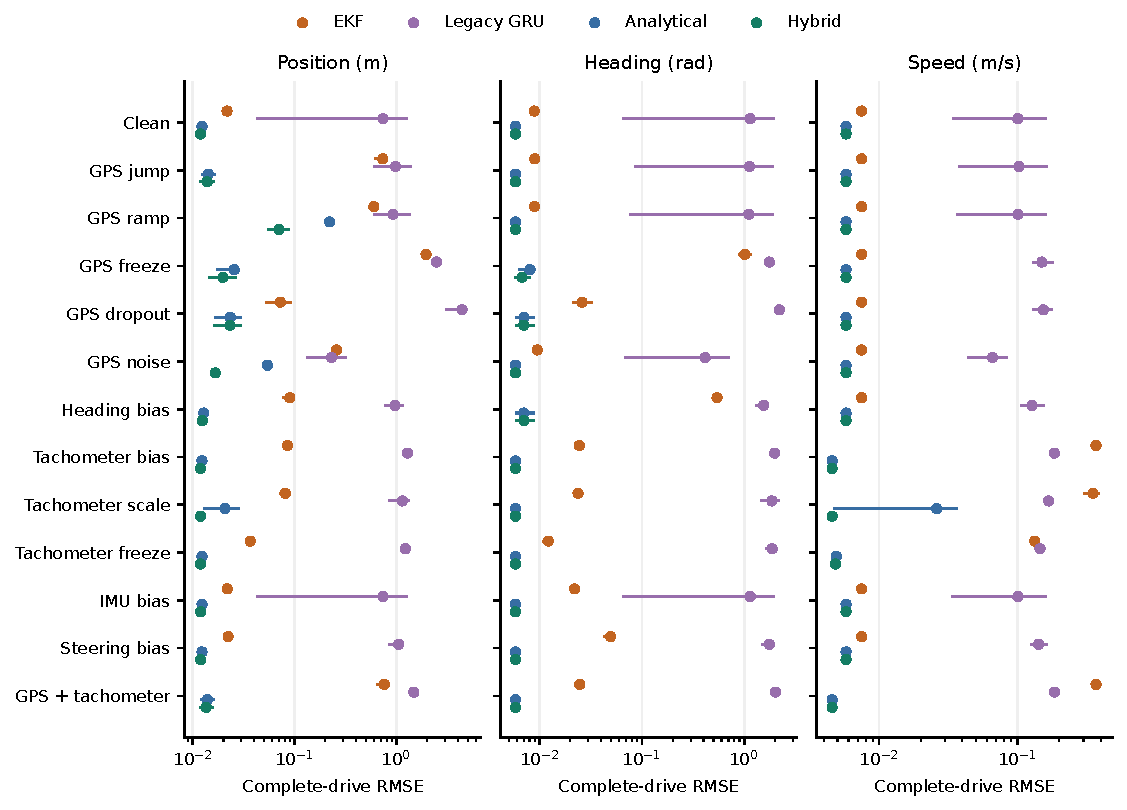
\includegraphics[width=\linewidth]{performance_overview.pdf}
\caption{Complete nominal benchmark: three seeds, 13 conditions and four estimators.
Dots show pooled RMSE and horizontal segments show the per-drive minimum--maximum range.
All panels use logarithmic error axes; lower is better. The legacy GRU is the retained
checkpoint, not an equally retrained architecture comparison.}
\label{fig:overview}
\end{figure}

\subsection{What learning contributes}
The ablation is essential for interpreting robustness. For GPS jumps, removing learning
changes position RMSE only from 0.0139 to 0.0142 m. Large jump rejection is therefore
predominantly explained by analytical design in this comparison.
For GPS ramp corruption, learning reduces error from 0.2202 to 0.0701 m, approximately
68.2\%. Under increased GPS noise the reduction is 0.0540 to 0.0166 m,
approximately 69.2\%. Tachometer scaling also benefits: speed RMSE decreases from
0.0261 to 0.0046 m/s. Figure~\ref{fig:relative} separates improvement over the EKF
from improvement over the analytical ablation. An entry of 0.10 means one tenth of
the reference RMSE, whereas 1.10 means 10\% more error. Values close to one indicate
little incremental benefit, even if both methods substantially outperform the EKF.

\begin{figure}[p]
\centering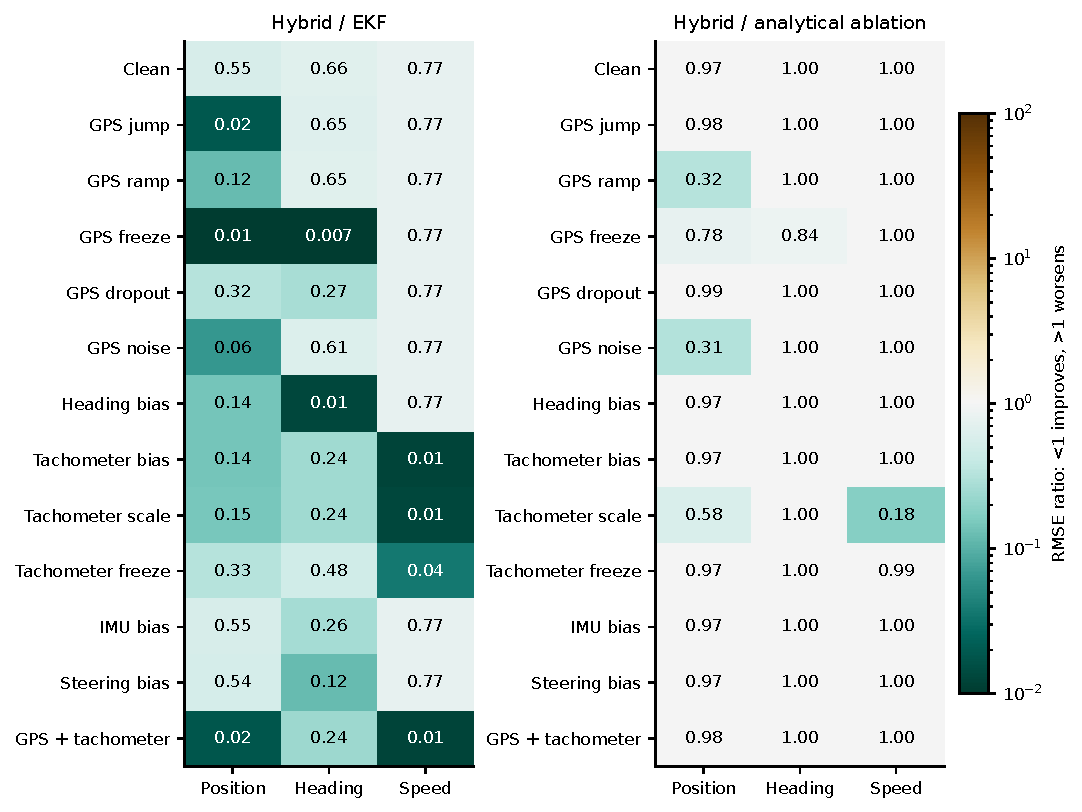
\includegraphics[width=\linewidth]{relative_performance.pdf}
\caption{Ratios of pooled nominal RMSE. Left: hybrid relative to EKF. Right: hybrid
relative to the analytical ablation. Values below one favor the hybrid; values above
one favor the comparator. Numerical labels give the ratios without color-scale clipping.
The logarithmic color scale is centered at equality and saturates outside $[0.01,100]$.
Learning's incremental effect is evaluated in the right-hand panel.}
\label{fig:relative}
\end{figure}

Figure~\ref{fig:trust} illustrates the trust factors for three corruptions of one drive.
Learned reliability and analytical consistency are distinct quantities; their
combination determines applied trust.
The shaded attack intervals are annotations supplied by the experiment for interpretation.
Online trust is inferred from sensor/model disagreement, not copied from those annotations.
The diagnostic replays are checked against the saved state trajectories before
the figures are generated. A low learned weight by itself is not the complete rejection
mechanism: availability, the analytical factor and GPS-coordinate coupling also matter.

\begin{figure}[htbp]
\centering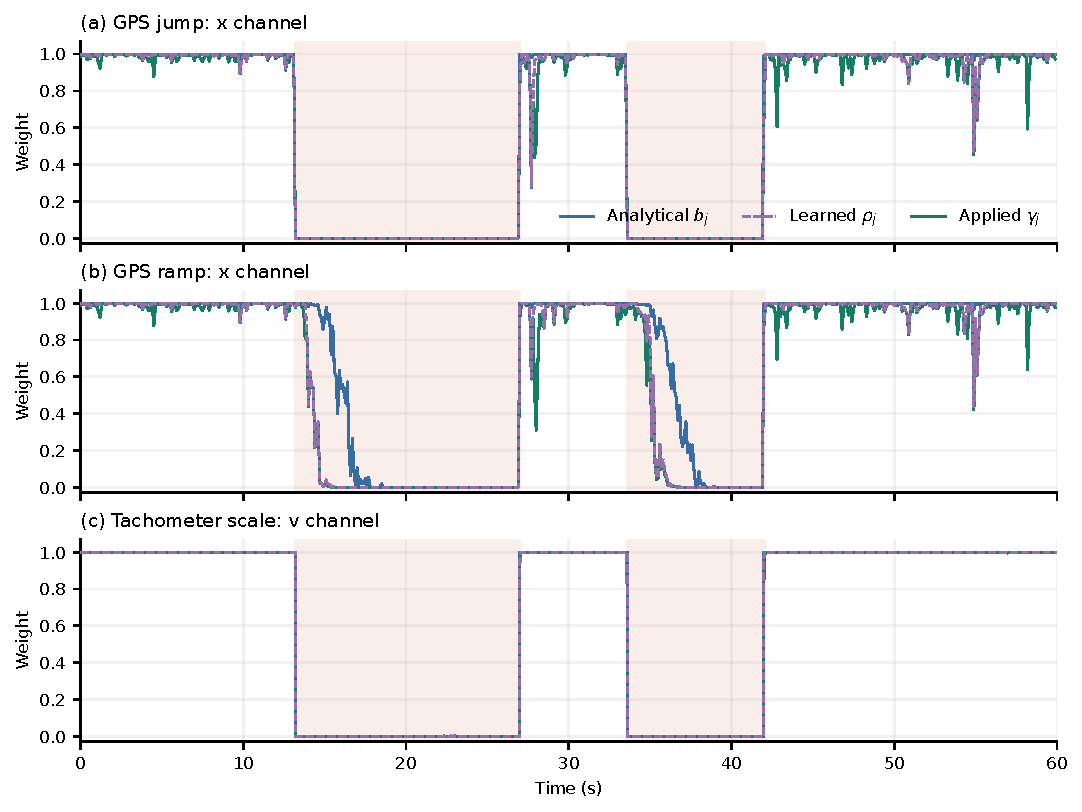
\includegraphics[width=.97\linewidth]{trust_factor_comparison.pdf}
\caption{Trust decomposition for seed 101: GPS jump ($x$), GPS ramp ($x$), and tachometer
scale corruption ($v$). Curves show analytical consistency $b_j$, learned reliability
$\rho_j$ and applied trust $\gamma_j$ at available measurements. Position trust includes
the minimum across both coordinates. Shading marks externally known injection intervals;
it is not a filter input. The analytical factor already strongly rejects large jumps.}
\label{fig:trust}
\end{figure}

\subsection{Observed masks, gains and observer outputs}
Figure~\ref{fig:masks} displays the actual four-channel applied mask, together with
GPS availability. A value near one permits a measurement correction; a value near zero
suppresses it. This is a reliability weight, not an attack probability or the simulator's
attack label. The heatmaps are sampled at the nominal GPS schedule, including missing
GPS slots. Plotting every 50 Hz step without this distinction would interleave ordinary
GPS non-arrival with rejected GPS and make a healthy asynchronous sensor look faulty.
The velocity row is sampled at the same display times, although it updates at 50 Hz.

The dropout panel illustrates a separate mechanism: $a^{GPS}=0$ forces pose trust to
zero even without classifying an attack. A GPS position jump instead arrives with
$a^{GPS}=1$; rejection follows from consistency and learned reliability. Equality of
the $x$ and $y$ rows follows from the implemented position-pair minimum. Heading and
speed are separately weighted, subject to their own evidence and guards.

\begin{figure}[p]
\centering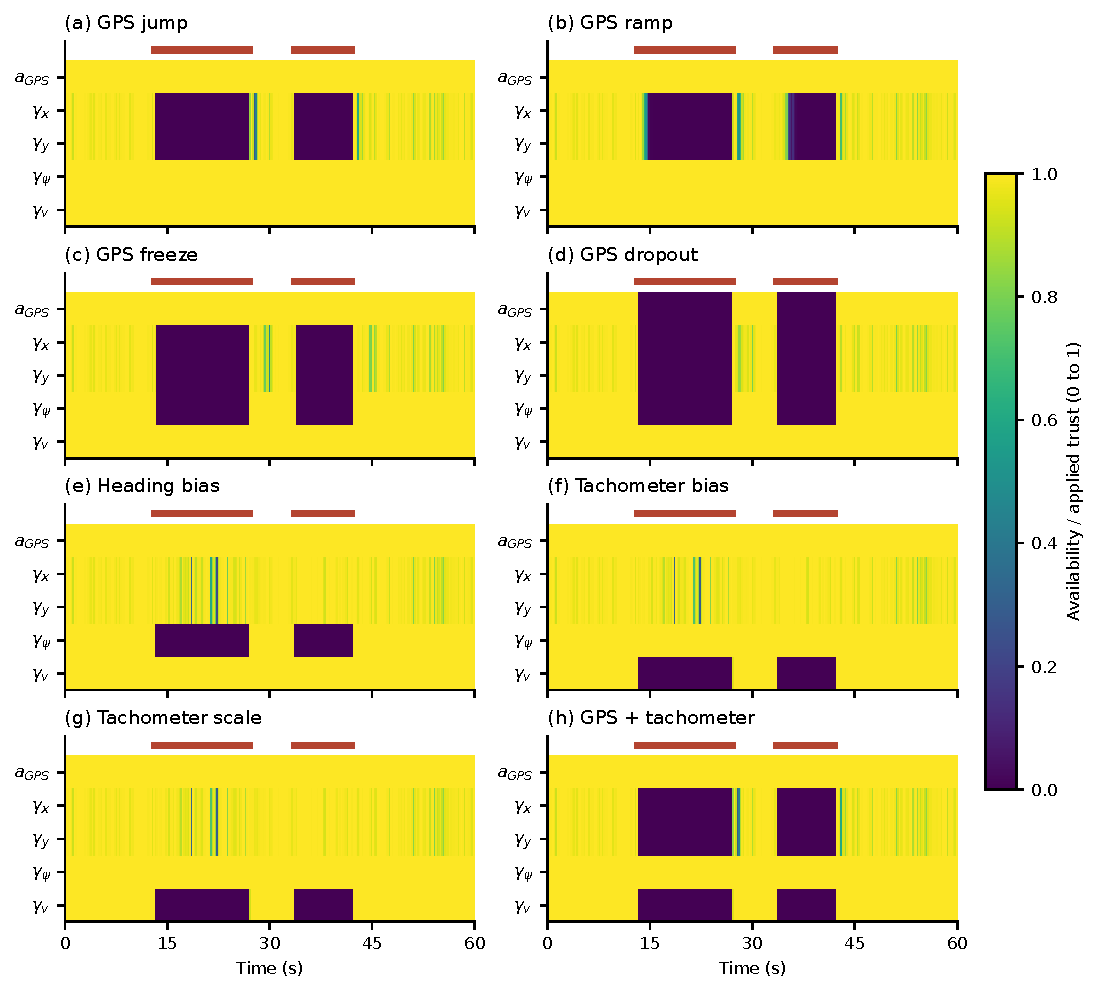
\includegraphics[width=\linewidth]{mask_channel_outputs.pdf}
\caption{Applied mask outputs for eight fault conditions on seed 101. Each panel has
one availability row and four trust rows, all on a common $[0,1]$ scale. Dark colors
mean unavailable or suppressed; bright colors mean available or highly trusted. Red
bars above the panels identify injection intervals only for interpretation. GPS slots
are shown at 10 Hz, including dropouts; velocity trust is subsampled for this display.
The first row distinguishes missing GPS from valid but rejected GPS.}
\label{fig:masks}
\end{figure}

The raw diagonal gain $K_j$ and the applied gain $\alpha_j=K_j\gamma_j$ must be
distinguished. Rejected updates can increase the variance-like quantity $P_j^-$ and
therefore increase raw $K_j$ while the applied gain remains near zero. A large raw gain
alone is consequently not evidence that an attack enters the state.
Figure~\ref{fig:gains} connects gain modulation to the actual correction and resulting
state error. For the hybrid, the plotted correction is $|\alpha_j r_j|$; for the EKF
it is $|(K^{EKF}r^{EKF})_j|$, including cross-channel terms. All methods use their own
prediction and residual. The comparison describes complete observers, not the isolated
effect of replacing one gain while holding all other states fixed.

\begin{figure}[p]
\centering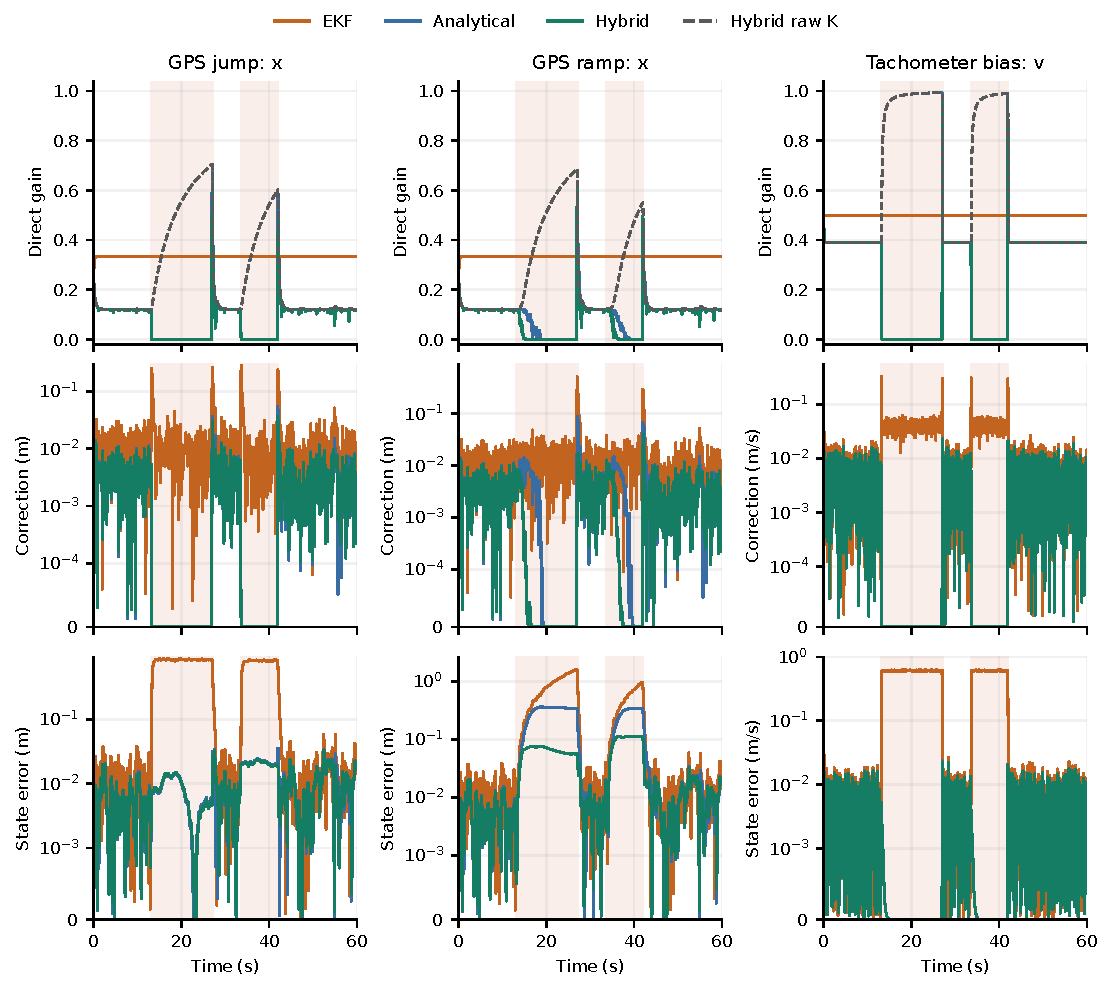
\includegraphics[width=\linewidth]{gain_correction_comparison.pdf}
\caption{From gain to correction to error, seed 101. Columns show GPS jump ($x$), GPS
ramp ($x$) and tachometer bias ($v$). Top: diagonal correction sensitivity for each
method; the dashed curve is the hybrid's raw $K_j$, and its solid green curve is the
applied $K_j\gamma_j$. Middle: magnitude of the complete measurement-induced state
correction. Bottom: absolute state error against truth. GPS gain/correction curves use
available GPS times; velocity curves use every step. Correction and error axes are
symmetric-log scales, with linear regions below $10^{-4}$ and $10^{-3}$ respectively
in the indicated units. Shading identifies injection intervals.}
\label{fig:gains}
\end{figure}

Figure~\ref{fig:gain_matrix} provides a complementary matrix view at the first attacked
GPS update. Since the state components have different units, the display uses
$D^{-1}KD$, where $D=\operatorname{diag}(0.12,0.12,0.09,0.10)$ contains the fixed feature
scales. For the hybrid and ablation, $K$ in this display means their effective correction
matrix unless explicitly labeled raw. This normalization makes matrix entries
dimensionless; it does not make the observers' priors or noise assumptions identical.
The matrix view exposes which residual can directly change which state component.
It does not quantify indirect coupling through subsequent predictions.

\begin{figure}[p]
\centering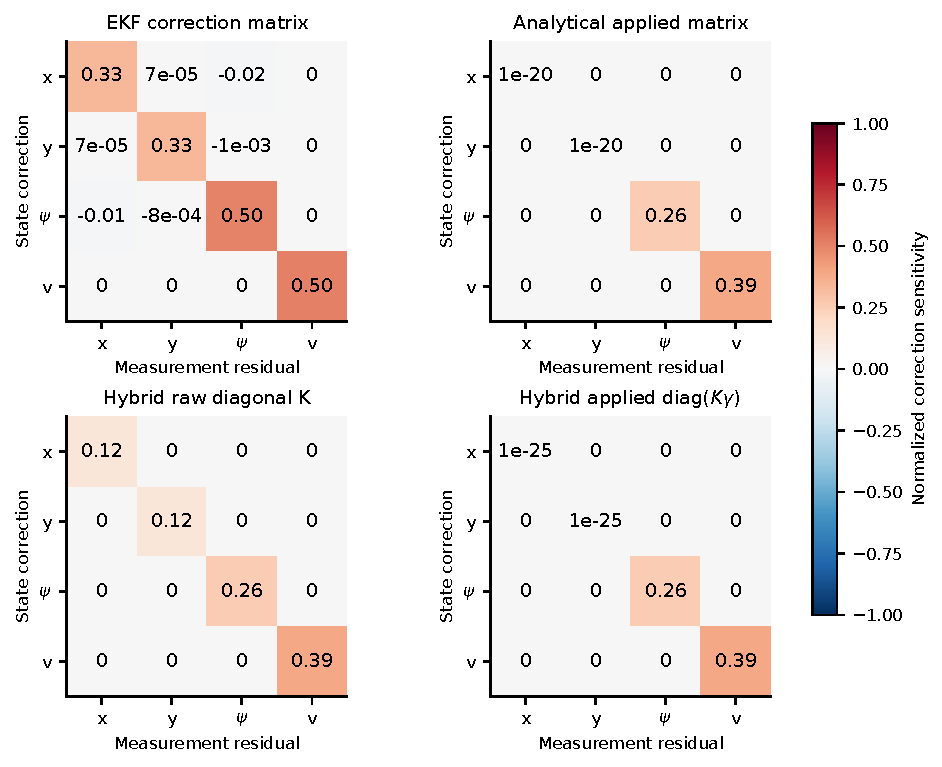
\includegraphics[width=.94\linewidth]{gain_matrix_snapshot.pdf}
\caption{Correction matrices at the first attacked GPS-jump sample, $t=13.2$ s,
seed 101. Rows are state corrections and columns are measurement residuals, normalized
by the stated fixed scales. Upper panels show the EKF and analytical ablation's applied
matrices. Lower panels separate the hybrid's raw diagonal gain from its mask-modulated
gain. Structural zero entries are labeled zero; tiny nonzero entries use scientific
notation. This is one diagnostic instant, not an average or a matrix-norm performance metric.}
\label{fig:gain_matrix}
\end{figure}

Figure~\ref{fig:states} then shows the four state outputs under simultaneous GPS and
tachometer corruption. Received measurements, simulator truth and observer outputs
are plotted together, and errors are shown separately so visually overlapping curves
can still be compared. The retained GRU is included in the error panels; omitting its
state excursions from the left-hand panels preserves the resolution of the other
outputs. The aggregate comparison in Fig.~\ref{fig:overview} includes all methods.

\begin{figure}[p]
\centering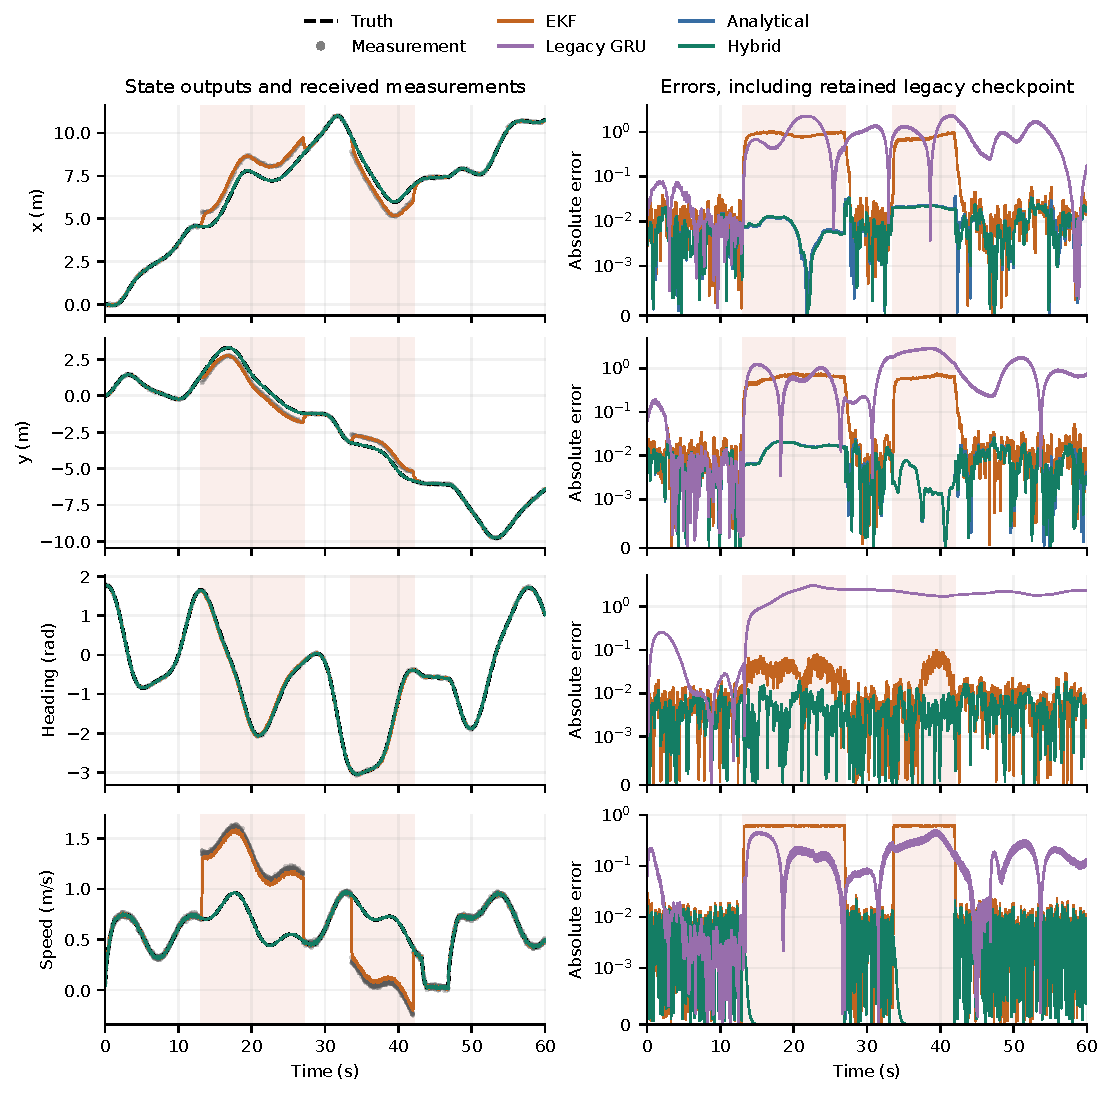
\includegraphics[width=\linewidth]{observer_state_comparison.pdf}
\caption{Observer outputs for combined GPS/tachometer corruption, seed 101. Left:
$x$, $y$, heading and speed, with true state (black dashed), corrupted measurements
(gray points) and three observer outputs. Right: absolute errors, including the legacy
GRU. Heading curves are expressed on the truth's unwrapped branch for readability;
heading errors are wrapped. Error axes use a symmetric-log scale with linear region
below $10^{-3}$ in each row's units. Shading identifies the externally defined attacks.}
\label{fig:states}
\end{figure}

\subsection{Attack-period and post-attack behavior}
Complete-drive averages alone can conceal a large error during corruption or delayed
recovery after its removal. Figure~\ref{fig:phases} therefore recomputes the same state
metrics using only attack samples and, separately, only the first 3 s after each attack.
For these 60 s drives the post-attack windows are $[27,30)$ and $[42,45)$ s.
The attack-only values reproduce the corresponding saved benchmark metrics. The
post-attack values are newly derived from the saved trajectories without rerunning or
retuning a filter. All three test seeds contribute to every reported ratio.
The hybrid has lower pooled error than the EKF in every displayed attack-period and
post-attack cell. This is evidence for these specified windows and fault conditions;
it is not a guarantee for arbitrary attack durations or recovery behavior.

\begin{figure}[p]
\centering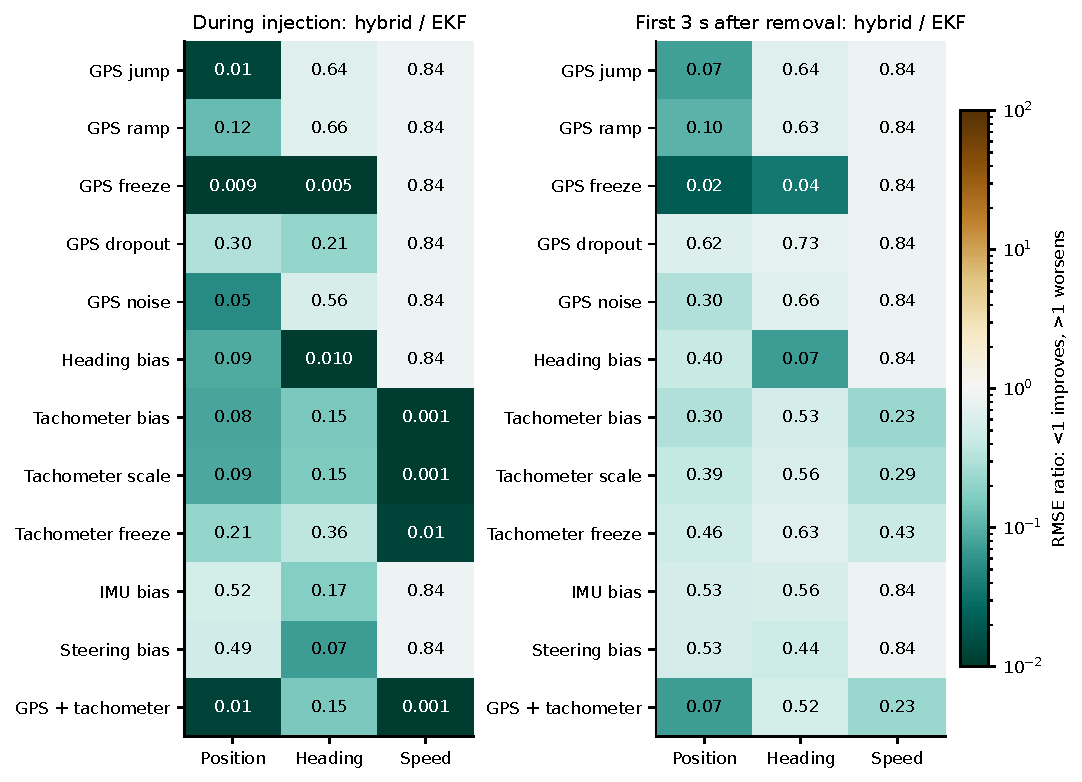
\includegraphics[width=\linewidth]{attack_recovery_performance.pdf}
\caption{Hybrid-to-EKF pooled RMSE ratios during injection (left) and in fixed 3 s
post-attack windows (right), for all 12 attacked nominal conditions and three seeds.
The clean condition is excluded because it has no injection/removal events. Ratios
below one favor the hybrid. Colors saturate outside $[0.01,100]$; numerical labels give
the values. A post-attack RMSE is not a settling-time estimate and can retain effects
of earlier state contamination.}
\label{fig:phases}
\end{figure}

\clearpage
\subsection{Closed-loop driving}
A separate benchmark uses the repository Stanley lateral controller and PID speed
controller. Each estimator drives its own MockQCar trajectory on a circle of radius
2 m with target speed 0.65 m/s. The vehicle starts at $(2,0,\pi/2)$, at rest.
Three seeds (401--403) run for 40 s at 50 Hz with 10 Hz noisy GPS.
The nine conditions in Table~\ref{tab:closed} use an attack interval $[10,24)$ s.
Fault definitions match Table~\ref{tab:faults} except that the GPS jump is fixed to
$(1,-0.7)$ m and applicable biases/ramps have positive sign.
Controller settings are recorded in Appendix~\ref{app:parameters}.

Path error is the absolute radial deviation $|\sqrt{x^2+y^2}-2|$.
Path and true-speed tracking RMSE exclude the first 3 s.
This radial metric measures departure from the reference circle, not along-track timing
or completion of an identical mission. Both path and speed must therefore be inspected.

\begin{table}[htbp]
\centering\small
\caption{Closed-loop radial path RMSE (m) and true-speed tracking RMSE (m/s),
pooled over three drives per condition after startup.}
\label{tab:closed}
\begin{tabular}{lrrrr}
\toprule
Condition & Path: EKF & Hybrid & Speed: EKF & Hybrid \\
\midrule
Clean & 0.0232 & 0.0227 & 0.0047 & 0.0057 \\
GPS jump & 0.4883 & 0.0249 & 0.0047 & 0.0057 \\
GPS ramp & 0.4388 & 0.0227 & 0.0047 & 0.0057 \\
GPS freeze & 1.7315 & 0.0231 & 0.0047 & 0.0057 \\
GPS dropout & 0.0257 & 0.0237 & 0.0047 & 0.0057 \\
Heading bias & 0.5005 & 0.0217 & 0.0047 & 0.0057 \\
Tachometer bias & 0.0194 & 0.0228 & 0.3651 & 0.0056 \\
Tachometer freeze & 0.0240 & 0.0228 & 0.0544 & 0.0057 \\
GPS + tachometer & 0.0465 & 0.0253 & 0.3651 & 0.0056 \\
\bottomrule
\end{tabular}

\end{table}
\begin{figure}[htbp]
\centering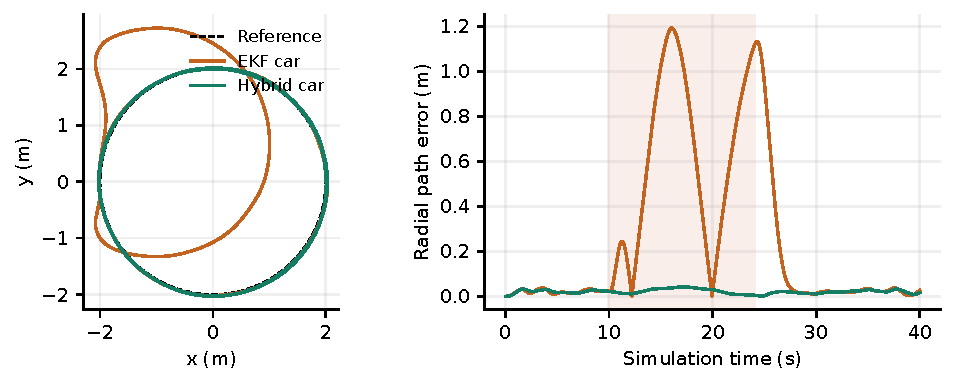
\includegraphics[width=.94\linewidth]{closed_loop_example.pdf}
\caption{GPS-jump driving example, seed 401. Left: separate true plant trajectories
under each estimator. Right: radial path error; shading marks the attack interval.
These are controlled-plant outputs, not two estimates of one common trajectory.}
\label{fig:closed}
\end{figure}

With a GPS jump, path RMSE decreases from 0.4883 m for the EKF-controlled car to
0.0249 m for the hybrid-controlled car. Under heading bias it decreases from 0.5005
to 0.0217 m. Not every path metric improves: under tachometer bias the EKF has slightly
lower radial error, 0.0194 versus 0.0228 m, but much worse speed tracking,
0.3651 versus 0.0056 m/s. That case illustrates why a single path metric can misrepresent
driving performance. This test exercises the estimator/controller/plant loop headlessly;
it does not validate the entire networked Ground Station execution stack.

\subsection{Calibration mismatch and a high-rate check}
A stress test uses seeds 201--202, 60 s drives, 5 Hz GPS, a plant time constant increased
by 20\%, and a steady-state speed curve increased by 10\%. The estimator retains nominal
calibration. Table~\ref{tab:stress} shows the harder combined-fault case explicitly.

\begin{table}[htbp]
\centering\small
\caption{Position RMSE (m) under plant-only calibration mismatch and 5 Hz GPS,
pooled over two drives. The analytical ablation outperforms the hybrid in the combined attack.}
\label{tab:stress}
\begin{tabular}{lrrr}
\toprule
Condition & EKF & Analytical & Hybrid \\
\midrule
Clean & 0.0265 & 0.0163 & 0.0158 \\
GPS ramp & 0.5919 & 0.1816 & 0.0709 \\
GPS dropout & 0.0659 & 0.0210 & 0.0201 \\
GPS + tachometer & 0.6571 & 0.4019 & 0.4638 \\
\bottomrule
\end{tabular}

\end{table}

Under simultaneous GPS and tachometer corruption, the hybrid gives 0.4638 m, below the
EKF's 0.6571 m but above the ablation's 0.4019 m. Rejecting the absolute measurement
leaves propagation dependent on an imperfect model; stronger rejection need not minimize
total trajectory error. This limits claims of universal benefit from learning.

Figure~\ref{fig:control_stress} places the complete closed-loop comparison beside the
calibration-mismatch experiment. It retains cases where the hybrid is worse on a
particular metric. In particular, the tachometer-bias path result and combined-fault
stress result should be considered alongside the gains in speed tracking and nominal
localization, rather than omitted from a visual robustness argument.

\begin{figure}[p]
\centering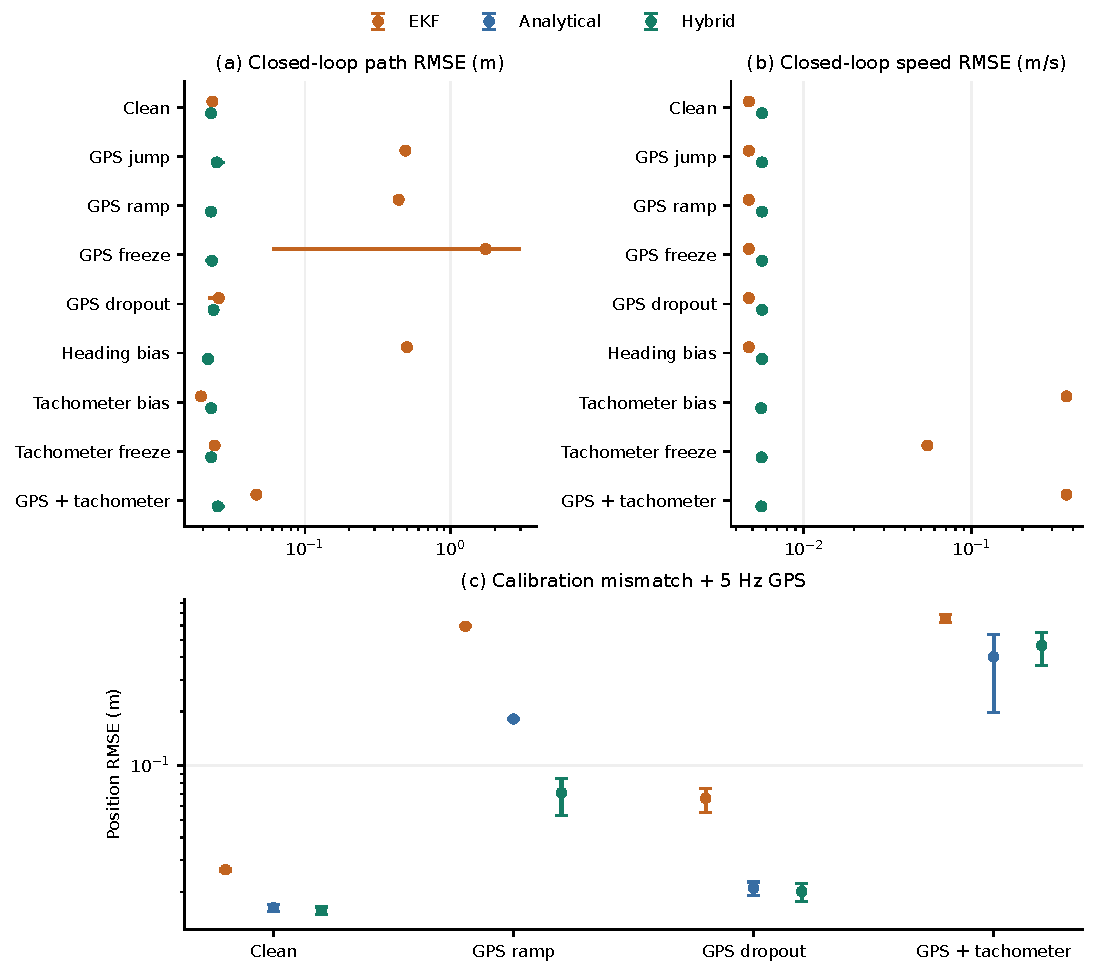
\includegraphics[width=\linewidth]{control_stress_comparison.pdf}
\caption{Driving performance and model-mismatch limits. (a,b) Closed-loop path and
speed tracking RMSE for all nine tested conditions, pooling three separate plant
trajectories per estimator and excluding startup. Dots show pooled RMSE and segments
span per-drive values. (c) Position RMSE under calibration mismatch and 5 Hz GPS, with
two seeds; error bars span those two values. All error axes are logarithmic. The
analytical ablation has lower combined-attack stress RMSE than the hybrid. Ranges
describe these observed drives and are not confidence intervals.}
\label{fig:control_stress}
\end{figure}

A separate one-seed check (203) uses 200 Hz estimation and GPS, 15 s drives, no added
sensor noise, and matched calibration. For GPS jump and dropout, hybrid position RMSE
is approximately $8.54\times10^{-5}$ and $1.37\times10^{-4}$ m.
These small values characterize a favorable near-matched simulation regime. They are
not evidence of corresponding physical-car localization accuracy.

\subsection{Computational cost}
Runtime evaluates the exported MLP with NumPy on CPU.
Table~\ref{tab:runtime} summarizes saved nominal timing observations.
For each estimator it reports the median of 39 per-drive medians and the median of
39 per-drive 95th percentiles; the latter is not a pooled p95 or a worst-case bound.

\begin{table}[htbp]
\centering\small
\caption{Saved estimator-update timing in the nominal benchmark.}
\label{tab:runtime}
\begin{tabular}{lrr}
\toprule
Method & Median trial median (ms) & Median trial p95 (ms) \\
\midrule
EKF & 0.405 & 0.670 \\
Legacy GRU & 6.792 & 8.471 \\
Analytical & 0.631 & 0.992 \\
Hybrid & 0.769 & 1.235 \\
\bottomrule
\end{tabular}

\end{table}

The hybrid is substantially cheaper than the retained GRU in this run, but slower than
the EKF. Measurements exclude the GUI, network bridge and full control-stack scheduling.
The original timing files do not contain a complete machine specification or load record,
so these values are descriptive rather than portable latency guarantees.
The high-rate check likewise does not establish a hard real-time deadline.

\section{Discussion and limitations}
The experiments support a practical division of responsibility. Calibrated propagation
and explicit guards handle several large or readily recognizable faults; learned trust
adds discrimination in cases such as gradual GPS displacement and excessive GPS noise.
Attributing the full EKF-to-hybrid improvement to the neural network would contradict
the ablation results.

Several limitations remain. First, the physical model and rejection scales are tuned to
the simulated QCar operating range. Sustained wheel slip, unexpected actuator dynamics or
noisy steering measurements can make correct observations look inconsistent.
Second, the auxiliary odometry reference can drift and can be indirectly influenced by
previous accepted corrections. It provides no independent absolute localization guarantee.
Third, the covariance-like recursion is heuristic; uncertainty calibration and probabilistic
coverage have not been measured.

The method suppresses unreliable information rather than reconstructing the attack
signal or identifying an attacker. Coordinated corruption that remains consistent with
the motion model may evade rejection. The available experiments use synthetic,
predefined faults, modest numbers of drives and known initial poses.
The fault set is shared between training and test, and the comparisons do not include a
separately tuned innovation-gated or robust-loss EKF. Such baselines are needed before
claiming an advantage over robust filtering generally.

No physical-car trials are reported here. The legacy GRU comparison is a checkpoint
comparison, not a controlled architecture comparison after equal retraining.
The study also lacks separate ablations for the anchor, individual guards and loss terms.
These limitations motivate tests with independently calibrated plants, unseen attack
mechanisms, additional robust baselines and physical sensor logs with an independent
position reference.

\section{Conclusion}
The revised RobustKLNet simulation backend combines physical prediction, analytical
consistency gates and learned measurement trust with diagonal correction gains.
It uses no online attack labels or clean sensor reference.
Continuous simulated estimation and closed-loop driving improve over the tested repository
EKF across many injected faults. The neural ablation shows where learning helps and where
the explicit analytical design already accounts for most of the robustness.
The observed failure under combined corruption and calibration mismatch remains part of
the result. The present evidence supports this hybrid implementation for the specified
simulation tests; broader robustness and transfer require further evaluation.

\section*{Reproducibility and evidence}
All reported primary metrics come from saved benchmark JSON/NPZ pairs in
\texttt{Robust/results}: \texttt{heldout}, \texttt{closed\_loop},
\texttt{stress\_mismatch}, and \texttt{native\_rate}.
The checkpoint is \texttt{models/innovation\_trust\_sim.npz}.
Its SHA-256 fingerprint is
\begin{center}\small\ttfamily
42fc0835b0f22c2f777ad7a9557ec2e0925\\
c85c5ddec1b7b8a289fb0d6851478
\end{center}
All four result files record that fingerprint.
The asset builder pools metrics directly from the saved per-drive rows, checks checkpoint
identity, and verifies 27 diagnostic rollouts (nine conditions, three observers,
seed 101) against saved trajectories to absolute tolerance $10^{-7}$.
Instrumentation observes the EKF's existing gain-reporting hook without replacing its
update equations. For every diagnostic step, the recorded prediction plus complete
gain--residual correction must reconstruct the returned state (including the runtime
adapter's float32 publication), and reconstructed availability/consistency/network
factors must match the applied mask.
The diagnostics and source fingerprints are retained in
\texttt{paper\_assets/observer\_diagnostics.npz} and its matching manifest.
Derived attack/post-attack metrics are saved in \texttt{phase\_metrics.json}; full-drive
comparison ratios are in \texttt{relative\_metrics.json}, in the same asset directory.
The expanded figure sets are exported as vector PDFs and reusable PNG images.
Source hashes are recorded in \texttt{paper\_assets/evidence\_manifest.json}.
This verifies artifact consistency, not historical provenance of every code revision.
The old mixed GRU/revision report is retained separately in \texttt{archive/}
and is not part of the current method description.

The dataset generator, training script, filter and benchmark scripts are included in the
project workspace. No public repository URL or public dataset release is asserted.
From the \texttt{Robust} directory, the relevant PowerShell commands are:
\begin{verbatim}
python train_robust_kalmannet.py --simulation-trust --epochs 60 --rounds 2
$ckpt = 'models/innovation_trust_sim.npz'
python validate_robust_kalmannet.py --simulation --duration 60 --legacy --checkpoint $ckpt
python closed_loop_benchmark.py
python -m unittest test_innovation_trust -v
\end{verbatim}
The validation command writes to \texttt{results/simulation\_metrics.json} by default;
the reported original run was saved as \texttt{results/heldout.json}.
Retraining and these output paths can replace associated local artifacts; a new checkpoint
must be identified by its own fingerprint.
The root-level \texttt{robust\_workflow.cmd} creates separate run folders and supports
headless evaluation, training and Ground Station web replay.
Replay displays completed benchmark trajectories; it does not alter the metrics or
stream the benchmark during computation.
To rebuild this manuscript, run \texttt{build\_paper\_assets.py} from its folder and then
run \texttt{pdflatex} twice on \texttt{robust\_kalmannet\_trust\_report.tex}.
Assets require the adjacent \texttt{../results} and \texttt{../models} directories.

\appendix
\section{Numerical settings}\label{app:parameters}
Nominal throttle/speed interpolation uses
\begin{align*}
\mathcal U&=[0,.04,.06,.08,.10,.12,.14,.16],\\
\mathcal V&=[0,.21971,.35357,.49205,.62316,.75836,.89438,1.02785]\ {\rm m/s}.
\end{align*}
Values are rounded here; the checkpoint and calibration YAML retain full precision.
The gain recursion uses
\begin{align*}
 \sqrt{\bm P_0}&=[.02,.02,.02,.04],&
 \sqrt{\bm Q}&=[.002,.002,.002,.006],&
 \sqrt{\bm R}&=[.035,.035,.015,.012],
\end{align*}
with state units in the order $[x,y,\psi,v]$ and $Q$ referenced to a 0.02 s step.
Valid estimator intervals satisfy $0<\Delta t\leq0.25$ s.
For the controller test, Stanley uses $k_e=2$, $k_{\rm soft}=0.2$,
a 0.13 m position lookahead offset and a 0.5 rad steering limit.
PID speed control uses $(k_p,k_i,k_d)=(0.12,0.25,0)$,
feedforward gain 0.16 and maximum throttle 0.16.
These are the evaluated settings, not optimized values for all controllers or vehicles.

\section{Deterministic guard details}\label{app:guards}
The steering actuator state $s^\delta_k$ obeys
\begin{equation}
 s^\delta_k=s^\delta_{k-1}+
 \Delta t_k\,\clip\big(10[\clip(\delta_k,-.52,.52)-s^\delta_{k-1}],-3,3\big),
\end{equation}
and the bicycle rate is
$\omega_k^{\rm bike}=\bar v_k\tan[(s^\delta_{k-1}+s^\delta_k)/2]/L$.
A non-finite steering sample retains the previous steering state.

A gyro fault latch is set when its successive finite values differ by more than
0.3 rad/s while successive steering signals differ by less than 0.05 rad.
It is cleared when $|\omega_k^{\rm IMU}-\omega_k^{\rm bike}|<0.12$ rad/s.
Subject to a clear latch and a finite gyro, the gyro is accepted if either its
discrepancy from the bicycle rate is below 0.3 rad/s or
$|a_k^{\rm IMU}-a_k^{\rm model}|<0.65$ $\mathrm{m/s^2}$.
Otherwise the bicycle rate is used.
The acceleration consistency term uses the acceleration returned by propagating the
command-driven auxiliary speed. These are implementation rules; an attacker is not
assumed to announce a gyro fault.

The tachometer freeze timer accumulates $\Delta t_k$ only while successive values
are exactly equal. Repetition for more than 0.15 s is rejected when
$\max(|v_k^{\rm tach}|,|v_k^{\rm cmd}|)>0.05$ m/s.
The feature-level repeated-value accumulator instead uses a difference threshold of
$10^{-7}$ and increments by the current interval since the last available GPS update,
lower-bounded by $\Delta t_k$, for each available channel.
It is therefore not a uniformly sampled physical freeze duration for all channels.
If both GPS position accumulators exceed 0.15 and $|v_k^{\rm use}|>0.08$ m/s,
the analytical terms for GPS position and GPS heading are zeroed.
This exact-freeze policy is suited to repeated packets in the tested simulator and
requires reassessment for quantized or noisy real sensors.

Availability follows per-channel finite checks and supplied position/heading
validity flags. It is not inferred from the simulator's attack indicator.
Between GPS packets, direct position and heading corrections are absent.
The main state, auxiliary reference, previous observations, discrepancy statistics,
timers and gyro latch are reset once at initialization of each drive.

\begin{thebibliography}{9}
\bibitem{revach2022}
G. Revach, N. Shlezinger, X. Ni, A. L\'opez Escoriza,
R. J. G. van Sloun, and Y. C. Eldar,
KalmanNet: Neural network aided Kalman filtering for partially known dynamics,
\emph{IEEE Transactions on Signal Processing}, vol. 70, pp. 1532--1547, 2022.
\href{https://doi.org/10.1109/TSP.2022.3158588}{doi:10.1109/TSP.2022.3158588}.
\bibitem{dahal2024}
P. Dahal, S. Mentasti, L. Paparusso, S. Arrigoni, and F. Braghin,
RobustStateNet: Robust ego vehicle state estimation for Autonomous Driving,
\emph{Robotics and Autonomous Systems}, vol. 172, article 104585, 2024.
\href{https://doi.org/10.1016/j.robot.2023.104585}{doi:10.1016/j.robot.2023.104585}.
\end{thebibliography}
\end{document}
